\documentclass[fontsize=12pt]{article}
\usepackage[a4paper, margin=1in]{geometry}
\usepackage{hyperref}
\usepackage{graphicx}

\title{\textbf{Figures from De Domenico \& Insolia 2012}}

\begin{document}
\maketitle
 
I have implemented the continuous loss approximation for UHECR proton energy losses during propagation based on the parameterisation in \cite{MD2012}. Here I summarise the results of reproducing a few of the figures from the original paper as a consistency check. 

\section*{Figure 2}

The losses of UHECR protons can be found by solving the following equation
\begin{equation}
\frac{\mathrm{d} E}{\mathrm{d} z} = - \frac{E}{L_\mathrm{loss}(z, E)}.
\end{equation}
$L_\mathrm{loss}$ is loss length in Mpc, given by
\begin{equation}
L_\mathrm{loss}(z, E) = \frac{\mathrm{d}z}{\mathrm{d}t} \frac{1}{\left[ \beta_\mathrm{rsh}(z) + \beta_\pi(z, E) + \beta_{e^{\pm}}(z, E) \right]},
\end{equation}
where the $\beta$ terms are the loss rates of the different processes, as defined in \cite{MD2012}. The original and created figures are shown in Figure~\ref{fig2comp}.

\begin{figure}
\centering
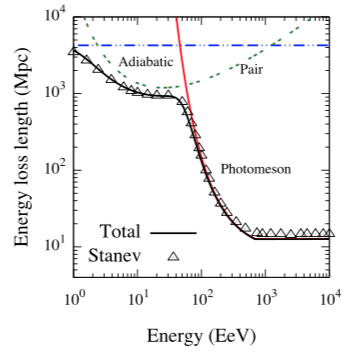
\includegraphics[width=0.5\textwidth]{figures/fig2_original.png}
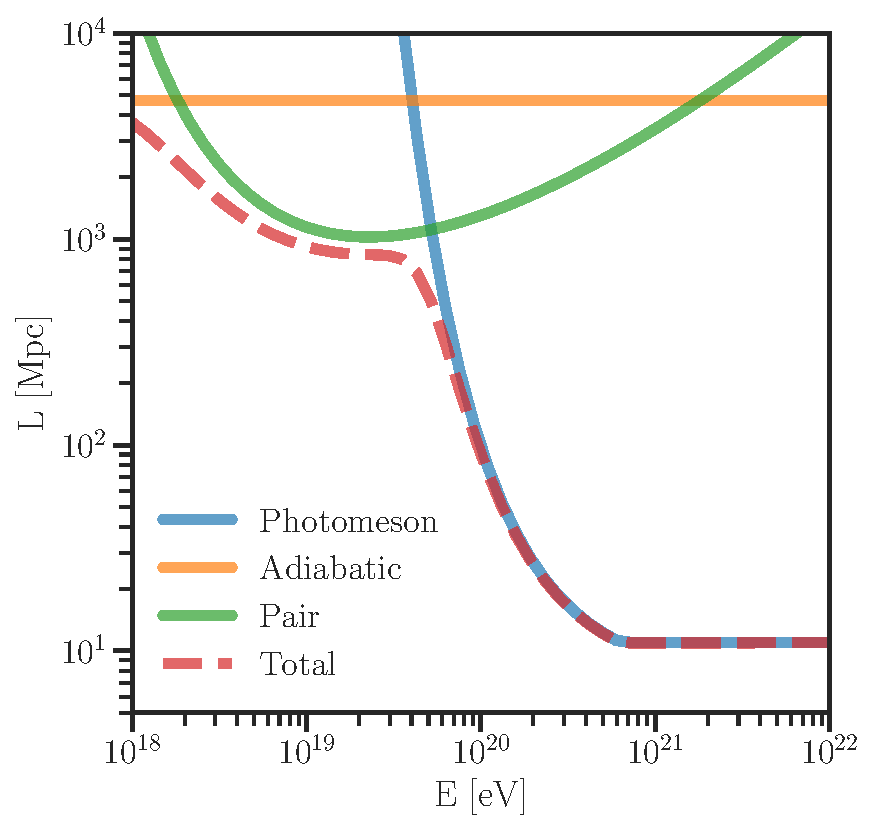
\includegraphics[width=0.5\textwidth]{figures/Fig2_MD2012.pdf}
 \caption{Comparison of Figure~2 from \cite{MD2012}. The original is shown on the top with the recreated underneath.}
 \label{fig2comp}
\end{figure}

\section*{Figure 4}

Following the notation of the original paper, the survival probability and flux of UHECR protons is given by (see Equations~10 and 11 in \cite{MD2012})
\begin{equation}
\omega_\mathrm{GZK}(z, E_f) = \frac{s-1}{E_f^{-s+1}} \int_{E_i(z, E_f)}^{\infty} E^{-s} \ \mathrm{d} E = \left[ \frac{E_i(z, E_f)}{E_f} \right]^{1 - s}
\label{omega}
\end{equation}
\begin{equation}
\Omega_{\mathrm{GZK}}(z, E_f) = \frac{\int_z^{\infty} \ \mathrm{d}z' \int_{E_i(z', E_f)}^{\infty} E^{-s} \ \mathrm{d}E }{\int_0^{\infty} \ \mathrm{d}z' \int_{E_i(z', E_f)}^{\infty} E^{-s} \ \mathrm{d}E }
\label{Omega}
\end{equation}

The original and recreated figures are shown in Figures~\ref{fig4acomp} and \ref{fig4bcomp}. Good agreement is found. \textbf{However, it should be noted that it is necessary to use $\omega_\mathrm{GZK}$ and not $\Omega_\mathrm{GZK}$, as described in the paper}. The same calculation for $\Omega_\mathrm{GZK}$ results in a different shape for the plotted quantities. 

\begin{figure}
\centering
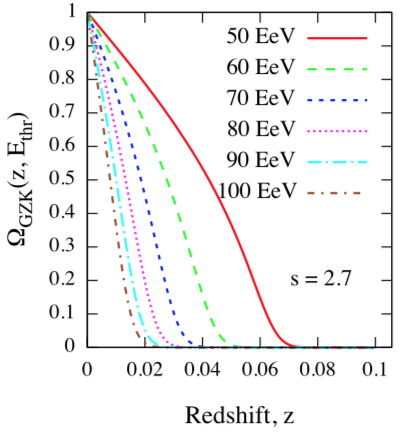
\includegraphics[width=0.5\textwidth]{figures/fig4a_original.png}
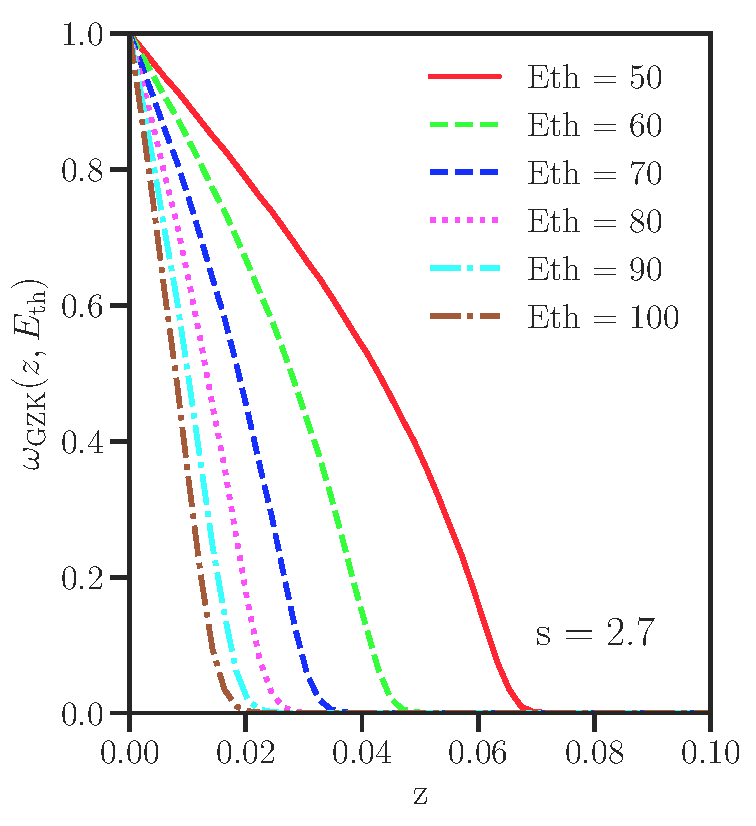
\includegraphics[width=0.5\textwidth]{figures/Fig4a_MD2012.pdf}
 \caption{Comparison of Figure~4a from \cite{MD2012}. The original is shown on the top with the recreated underneath.}
 \label{fig4acomp}
\end{figure}

\begin{figure}
\centering
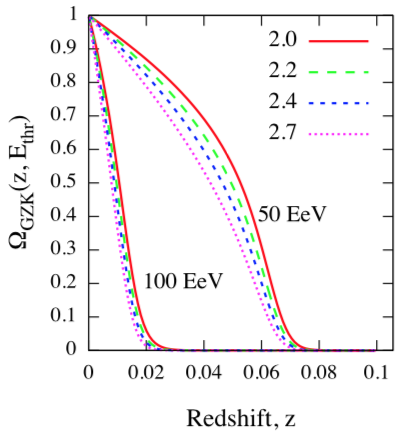
\includegraphics[width=0.5\textwidth]{figures/fig4b_original.png}
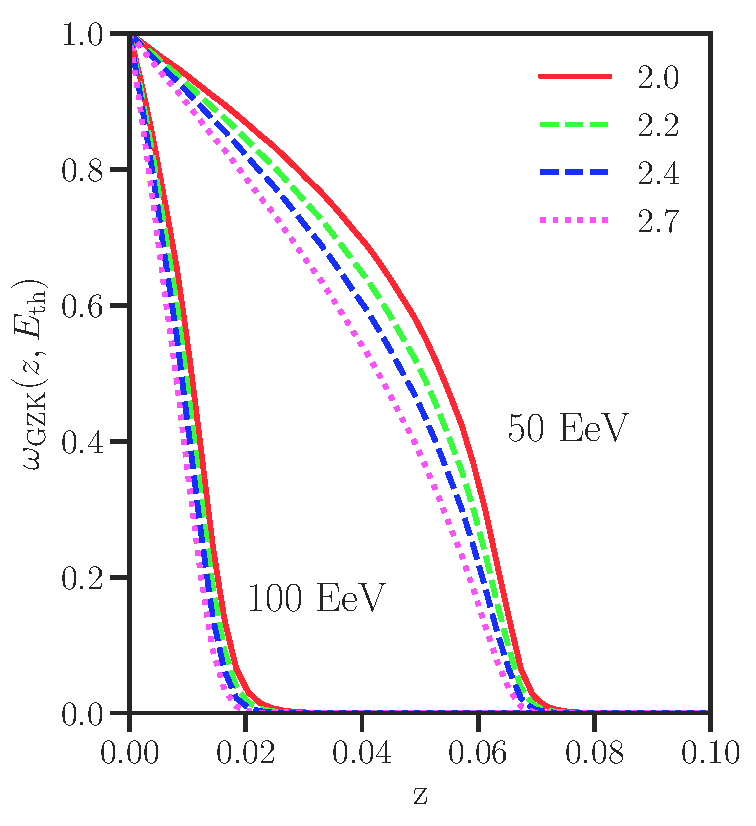
\includegraphics[width=0.5\textwidth]{figures/Fig4b_MD2012.pdf}
 \caption{Comparison of Figure~4b from \cite{MD2012}. The original is shown on the top with the recreated underneath.}
 \label{fig4bcomp}
\end{figure}


\begin{thebibliography}{9}

\bibitem{MD2012} 
De Domenico, M. \& Insolia, A., 2012. \emph{Influence of cosmological models on the GZK horizon of ultrahigh energy protons}. Journal of Physics G: Nuclear and Particle Physics, 40(1), p.015201.

\end{thebibliography}


\end{document}

